Este capítulo describe el componente de software desarrollado para que las aplicaciones interactúen de forma autónoma con el dron. Es responsable de acceder a los sensores y actuadores del vehículo utilizando los mensajes de comunicación del protocolo MAVLink, y de traducirlos a las interfaces ICE de JdeRobot. Las aplicaciones de drones tendrán acceso a los sensores y actuadores del vehículo a través de esas interfaces.

La comunicación de nuestro driver con el dron es bidireccional. Dependiendo del módulo que se esté usando, esta comunicación puede ser bien dron-servidor, como por ejemplo recoger coordenadas GPS, bien servidor-dron, por ejemplo para ordenar comandos de velocidad, o bien bidireccional, para realizar la conexión con el servidor y envío de ACKs. 

\begin{figure}[H]
  \hspace*{-3.5cm}
  
\includegraphics[scale=0.5]{imagenes/muySencillo.png}
  \caption{Diagrama comunicación}
  \label{fig:diagramaComunicacionServerDron1}
\end{figure}

\section{Diseño}
\label{Diseno}

\texttt{MAVLinkServer} es un driver basado en el software MAVProxy y desarrollado para actuar como un \textit{middleware} de traducción. Ha sido diseñado como un controlador JdeRobot en lenguaje Python. Es responsable de mantener los canales de comunicación abiertos y actualizados, tanto en sentido ascendente como descendente. 

En la imagen \ref{fig:diagramaHwSw} se indica cómo es la relación entre el hardware y el software de cada componente, así como la comunicación interna o la comunicación hacia otros elementos.

\begin{figure}[H]
  \centering
  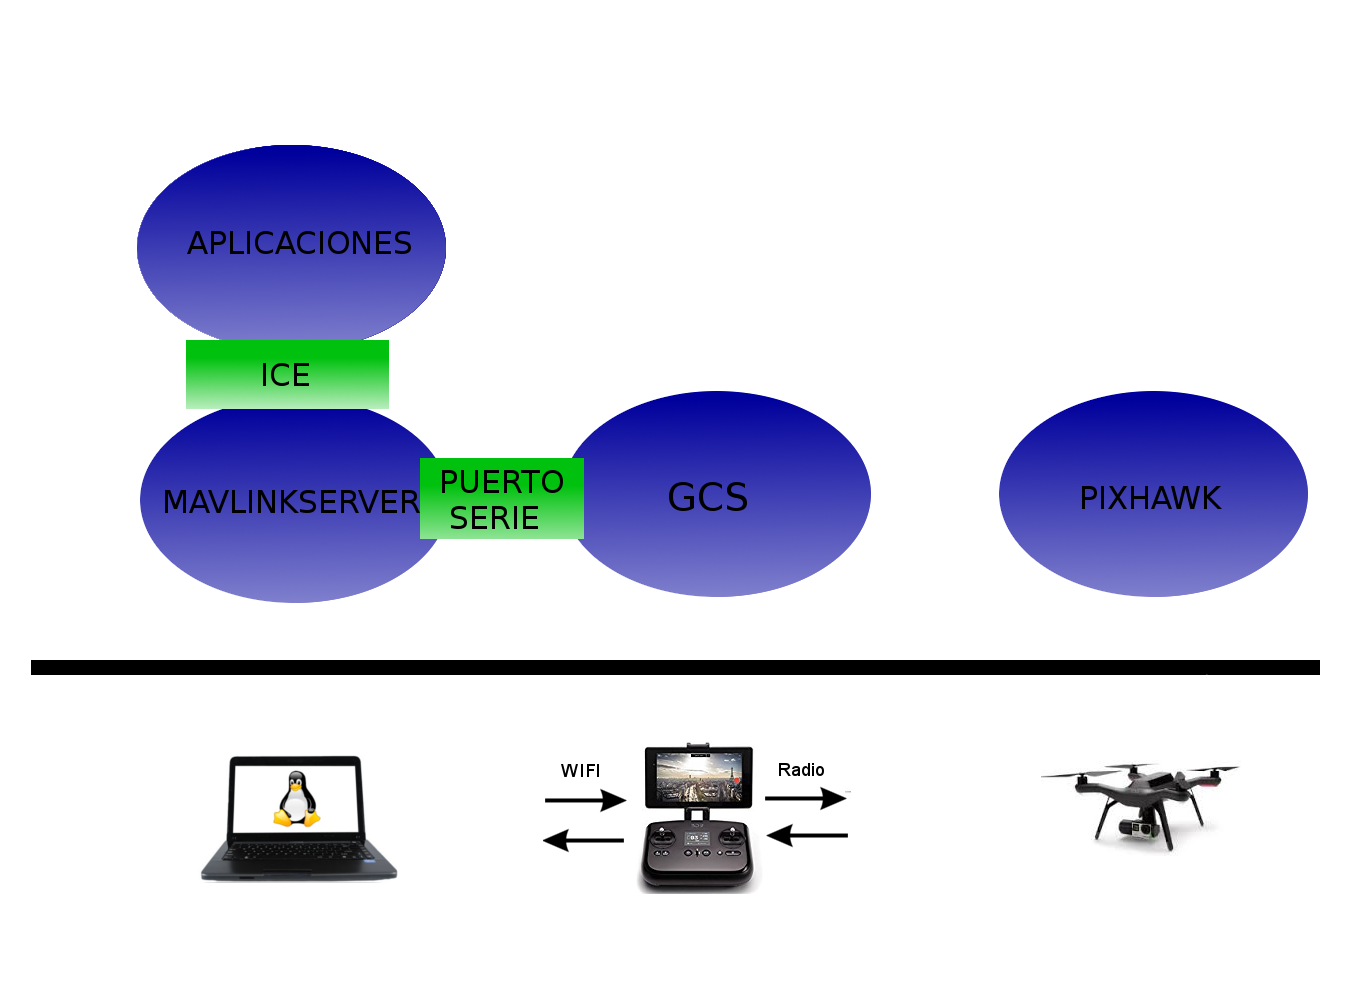
\includegraphics[scale=0.3]{imagenes/HWYSW.png}
  \caption{Diagrama de Hardware y Software}
  \label{fig:diagramaHwSw}
\end{figure}

El driver se ha diseñado combinando tres bloques como se indica en la figura \ref{fig:memoriaCompartida}: el de configuración; el de diálogo con el drone usando MAVProxy; y el de diálogo con la aplicación usando interfaces ICE.

\begin{figure}[H]
  \centering
  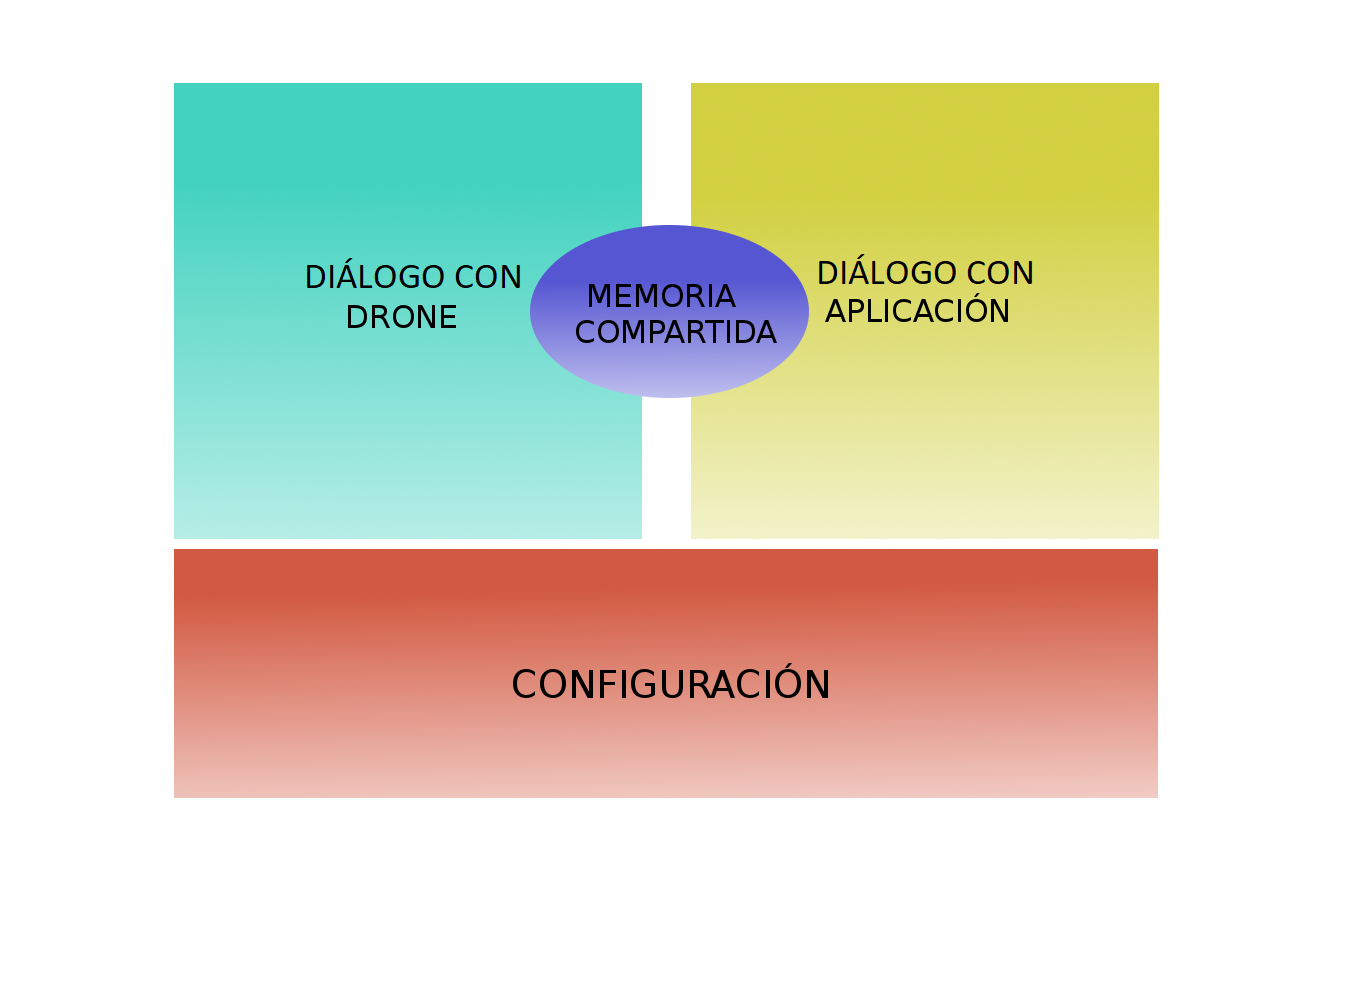
\includegraphics[scale=0.25]{imagenes/MEMORIACOMPARTIDA.png}
  \caption{Diagrama de bloques en MAVLinkServer}
  \label{fig:memoriaCompartida}
\end{figure}

El primer bloque es el que realiza la configuración necesaria para preparar todas las conexiones de los dos bloques siguientes. Toda la configuración se realiza a través de un único fichero para las interfaces ICE, ya que los módulos que se quieran añadir adicionalmente, se deben introducir mediante argumentos en la ejecución del script de arranque.

En el segundo bloque, \texttt{MAVLinkServer} establece la conexión con el piloto automático Pixhawk a bordo del drone, mantiene el canal de comunicación operativo, adquiere, interpreta, crea y envía mensajes nuevos con la información solicitada u ordenada por la aplicación.

El código desarrollado en tercer bloque, está principalmente a cargo de la gestión de las interfaces ICE de JdeRobot. Es capaz de manejar la información proporcionada por el lado de MAVProxy. Regula la creación y modificación de las clases donde la información se almacena temporalmente y abre canales de comunicación ICE para hacer que el driver sea utilizable para aplicaciones JdeRobot.

Estos tres bloques en conjunto proporcionan un driver fiable y multi-compatible; \texttt{MAVLinkServer} puede conectarse con aplicaciones escritas en otros lenguajes, como C++, Python o Java, a través de las interfaces ICE de JdeRobot. La figura \ref{fig:mavLinkJdeRobotNegra} representa un esquema de entradas y salidas dentro de \texttt{MAVLinkServer} y sus conexiones a otras aplicaciones.


\begin{figure}[H]
  \centering
  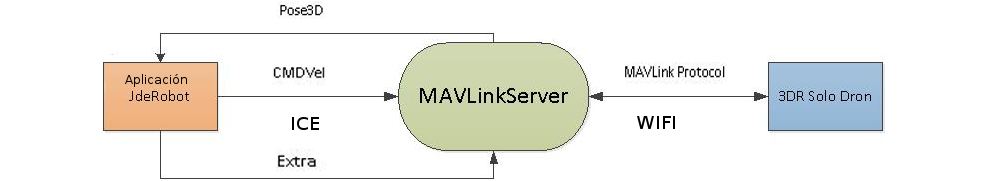
\includegraphics[scale=0.65]{imagenes/cajaNegraNueva.png}
  \caption{Diagrama de entradas y salidas bloques MAVLinkServer}
  \label{fig:mavLinkJdeRobotNegra}
\end{figure}

La información que se maneja dentro del driver se gestiona a través de memoria compartida. Es necesario que la información sea bidireccional y que la memoria se esté leyendo y escribiendo de la manera más ágil posible. Todas estas acciones se realizan mediante semáforos de exclusión mutua que permiten un acceso seguro y sin condiciones de carrera. Por ejemplo, obtener la información de los sensores del dron, informar a la aplicación de su situación y que concurrentemente la aplicación envíe las acciones que debe realizar el dron sin que ninguna de dichas acciones se vea afectada por la otra.

\begin{figure}[H]
  \centering 
  \hspace*{-2.5cm}     
  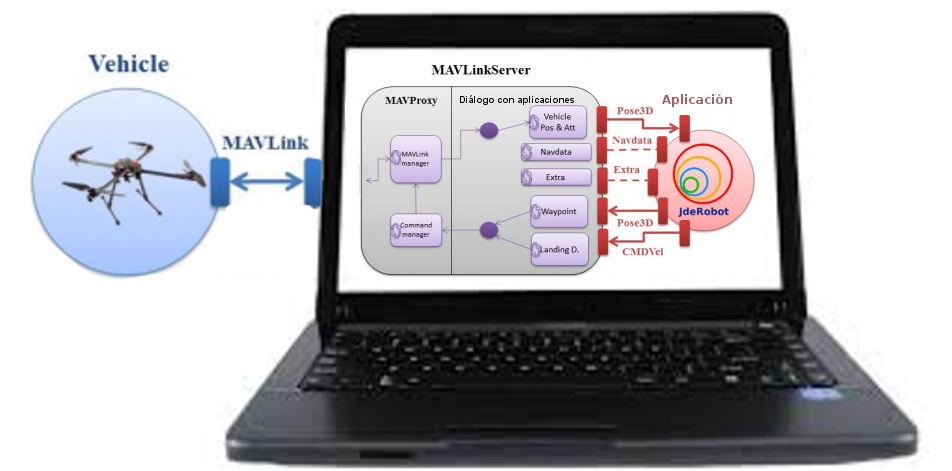
\includegraphics[scale=0.45]{imagenes/cajaTransparente.png}
  \caption{Diagrama bloques MAVLink-JdeRobot con detalle}
  \label{fig:mavLinkJdeRobotTrasparente}
\end{figure}

Las interfaces JdeRobot utilizadas en este proyecto se muestran en la figura \ref{fig:MavProxyInside} son \texttt{Pose3D} (proporciona la posición y medidas del vehículo), \texttt{CMDVel} (para enviar los comandos de velocidad) y \texttt{Extra} (para despegue y aterrizaje).

\begin{figure}[H]
  \centering
  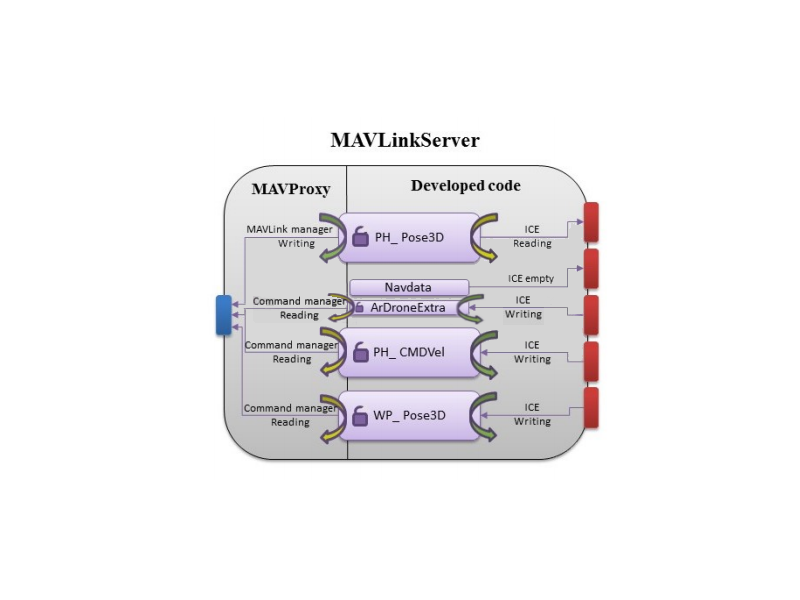
\includegraphics[scale=0.45]{imagenes/MavProxyPorDentro.png}
  \caption{Diagrama de bloques de MavLinkServer}
  \label{fig:MavProxyInside}
\end{figure}


\section{Diálogo con drone vía MavProxy}
Antes de que el driver pueda ejecutar correctamente hay que configurar el software \texttt{MAVProxy} del sistema. En este apartado vamos a explicar todos los pasos a seguir.

\subsection{Configuración}
\label{Pre-Configuracion}
Para configurar \texttt{MAVProxy} debemos tener en cuenta de una serie de ficheros, llamados módulos,  cada uno de los cuales facilita una utilidad diferente. Pueden ir desde conocer la batería, la altura del dron o configurar una web-cam.

Estos módulos se pueden descargar desde el repositorio oficial de \texttt{MAVProxy}\footnote{\url{https://github.com/ArduPilot/MAVProxy}} o crear una librería propia e implementarla. Los módulos que se han usado en este TFG para la comunicación vía \texttt{MAVProxy} son: 

\begin{itemize}
\item \texttt{mavproxy\_link}: Realiza la interconexión entre dron y MAVLinkServer.
\item \texttt{mavproxy\_arm}: Necesario para el despegue.
\item \texttt{mavproxy\_cmdlong}: Envía los comandos de velocidad al dron y órdenes de despegue y aterrizaje.
\item \texttt{mavproxy\_console}: Intérprete de comandos desde la consola de texto.
\item \texttt{mavproxy\_sensors}: Recoge información de los sensores.
\end{itemize}

\subsection{Inicialización}
El script de arranque se encarga de ejecutar todos los comandos preparatorios para \texttt{MAVProxy} y de lanzar el servidor. El script se encuentra en MAVProxy/MAVProxyWinLAN.sh. Antes de ejecutarlo debemos averiguar la IP que levanta el dron (en nuestro caso, con el 3DR Solo, dicha IP la levanta el mando) y modificar el script con la IP del dron. Una vez retocado hay que ejecutarlo sin parámetros adicionales. 

Se necesita tener preinstalado tanto \texttt{pyserial} como una versión de \texttt{pyvmavlink} superior a la 1.1.50. Se realiza una descarga de todos los módulos, construye un directorio llamado MavProxy.egg en /home/USER/.local/python2.7/site-packages con el fin de tener almacenados todos los paquetes necesarios y con permisos suficientes. 

La configuración que se puede modificar en el script de arranque está relacionada con el tipo de conexión que se quiere mantener con el dron. Esta conexión tiene valores por defecto pero se puede modificar si así se desea. Los comandos que se muestran en la tabla 4.1 son un ejemplo de la versatilidad que tiene el servidor. A través de los módulos descargados es posible acceder a los comandos que proporciona MAVLink. A continuación se proporciona un listado de los posibles comandos opcionales que se pueden añadir al script de arranque y una breve explicación de cada uno de ellos en la tabla 4.1:

\begin{center}
  \label{tab:scriptArranqueComandos}
  \begin{tabular}{ | l | p{7cm} | p{3.5cm} |}
    \hline
    \textbf{Comando} & \textbf{Acción} & \textbf{Valor por defecto} \\ \hline
    master & Puerto maestro MAVLink y baudrate opcional &  \\ \hline
    udp & Arranca el servidor udp & TCP \\ \hline
    tcp & Arranca el servidor tcp & TCP \\ \hline
    out & Puerto de salida MAVLink & \\ \hline
    baudrate & & 57600  \\ \hline
    sitl& Puerto de salida, esta opción únicamente es necesaria en caso de no tener disponible un dron.& \\ \hline
    streamratedest &  MAVLink stream rate & 4 \\ \hline
    source-system & Código fuente MAVLink & 255 \\ \hline
    source-component & Componente origen MAVLink & 0 \\ \hline
    target-system & Sistema destino MAVLink & 0  \\ \hline
    target-component & Componente destino MAVLink & 0 \\ \hline
    logfile & Fichero de logs & mav.tlog \\ \hline
    append-log & Añadir al fichero de log ya existente & False  \\ \hline
    continue & Continua el log& False \\ \hline
    quadcopter& Usar acciones de control para cuadricopteros&  False\\ \hline
    setup& Arrancar en modo setup & False \\ \hline
    nodtr& Deshabilitar DTR(Data Terminal Ready) & False \\ \hline
    show-errors& Mostrar errores MAVLink& False \\ \hline
    speech& Usar texto para hablar & False \\ \hline
    aircraft& Establecer nombre para el dron (Visual en mensajes)& None \\ \hline
    cmd& Comandos a ejecutar tras el arranque & None  \\ \hline
    console& Usar consola GUI para introducir comandos &  \\ \hline
    map& Carga un mapa de la zona&  \\ \hline
    load-module& Carga un modulo especifico, puede ser utilizado tantas veces como sea necesario separando con ",")&  \\ \hline
    mav09& Usa protocolo MAVLink 0.9 & False \\ \hline
    auto-protocol&Auto detecta versión de protocolo MAVLink& False \\ \hline
  \end{tabular}
  \captionof{table}{Tabla de comandos de arranque}
\end{center}
\begin{center}
  \label{tab:scriptArranqueComandos2}
  \begin{tabular}{ | l | p{7cm} | p{3.5cm} |}
  \hline
    \textbf{Comando} & \textbf{Acción} & \textbf{Valor por defecto} \\ \hline
    nowait&No realiza comunicación continua con el dron (HearthBeat) &  False\\ \hline
    dialect & Dialecto MAVLink& ardupilotmega \\ \hline
    rtscts& Habilita control de comunicación vía RTS/CTS&  False\\ \hline
    mission& Nombre de la misión& None \\ \hline
    daemon & Arranca en modo daemon, no muestra shell interactiva & False \\ \hline
    profile& Arranca el Yappi python profiler& False \\ \hline
    state-basedir& Directorio base para logs& None \\ \hline
    version& Muestra información sobre la versión& False \\ \hline
    default-modules& Módulos por defecto al iniciar.& log, wp, rally, fence, param, relay, tuneopt, arm, mode, calibration, rc, auxopt, misc, cmdlong, battery, terrain, output \\ \hline
  \end{tabular}
\end{center}

Todos los módulos se cargan mediante una importación de paquetes. La lista que se carga mediante este procedimiento se divide en los módulos que se cargan por defecto, como pueden ser el que \texttt{link} o \texttt{sensors}, y otros opcionales que se pueden seleccionar desde la configuración, como por ejemplo \texttt{console}. A continuación se muestra la función que permite esta carga:
\begin{lstlisting}[frame=single]

def load_module(modname, quiet=False):
    '''load a module'''
    modpaths = ['MAVProxy.modules.mavproxy_%s' % modname, modname]
    for (m,pm) in mpstate.modules:
        if m.name == modname:
            if not quiet:
                print("module %s already loaded" % modname)
            return False
    for modpath in modpaths:
        try:
            m = import_package(modpath)
            imp.reload(m)
            module = m.init(mpstate)
            if isinstance(module, mp_module.MPModule):
                mpstate.modules.append((module, m))
                if not quiet:
                    print("Loaded module %s" % (modname,))
                return True
            else:
                ex = "%s.init did not return a 
                      MPModule instance" % modname
                break
        except ImportError as msg:
            ex = msg
            if mpstate.settings.moddebug > 1:
                import traceback
                print(traceback.format_exc())
    print("Failed to load module: %s. Use 'set moddebug 3' 
         in the MAVProxy console to enable traceback" % ex)
    return False
\end{lstlisting}


\subsection{Funcionamiento continuo}

Para llevar a cabo esta preparación el primer módulo que se carga es "Link", este paquete se encarga de la conexión entre el servidor y el dron. Es necesario conocer la dirección IP que levanta este dron, que ya habremos configurado en el paso \ref{Pre-Configuracion}.

Tras lograr la conexión se establece un periodo de chequeo necesario para no perder la conexión con el dron en caso de llegar a una distancia límite o un fallo de conexión, en cuyo caso se procede a detener el dron. Periódicamente se debe realizar una comunicación entre el dron y el servidor, aunque no se llegue a mandar ningún comando, ya sea de velocidad o algún tipo de acción. El servidor por su parte comunicará que aún está conectado. Después de un tiempo sin conexión, aproximadamente unos 10-15 segundos, el dron procederá a realizar un aterrizaje. 

\begin{lstlisting}[frame=single]
def periodic_tasks():
    '''run periodic checks'''
    if mpstate.status.setup_mode:
        return
    if (mpstate.settings.compdebug & 2) != 0:
        return

    if mpstate.settings.heartbeat != 0:
        heartbeat_period.frequency = mpstate.settings.heartbeat

    if heartbeat_period.trigger() and mpstate.settings.heartbeat != 0:
        mpstate.status.counters['MasterOut'] += 1
        for master in mpstate.mav_master:
            send_heartbeat(master)
    if heartbeat_check_period.trigger():
        check_link_status()

    set_stream_rates()

    for (m,pm) in mpstate.modules:
        if hasattr(m, 'idle_task'):
            try:
                m.idle_task()
            except Exception as msg:
                if mpstate.settings.moddebug == 1:
                    print(msg)
                elif mpstate.settings.moddebug > 1:
                    exc_type, exc_value, exc_traceback = sys.exc_info()
                    traceback.print_exception(exc_type, exc_value, 
                    		exc_traceback,limit=2, file=sys.stdout)

        # also see if the module should be unloaded:
        if m.needs_unloading:
            unload_module(m.name)
\end{lstlisting}

En el lado de comunicación con el cuadricóptero, el driver sólo tiene una conexión con el dron a través de una IP y un puerto que se especifican en el arranque. Este bloque de \texttt{MAVLinkServer} está programado con tres hilos separados, uno para cada información relevante a intercambiar con el dron: posición, comandos de velocidad y comandos extra. La gestión de estos 3 hilos, respecto al único puerto abierto con el dron, se basa en prioridades. El hilo de comandos Extra predomina sobre los otros 2 debido a la importancia de las órdenes que envía. El segundo hilo prioritario es el que envía los comandos de velocidad. El hilo menos prioritario es el de recepción de actualizaciones de posición. 

\begin{lstlisting}[frame=single]
    mpstate.status.thread = threading.Thread(target=main_loop, 
    						name='main_loop')
    mpstate.status.thread.daemon = True
    mpstate.status.thread.start()

    # Open an MAVLink TX communication and 
    # leave it open in a parallel thread
  
    PoseTheading = threading.Thread(target=sendCMDVel2Vehicle, 
    				args=(PH_CMDVel,PH_Pose3D,), 
                    name='TxCMDVel_Theading')
    PoseTheading.daemon = True
    PoseTheading.start()

    # Open an MAVLink TX communication and 
    # leave it open in a parallel thread

    PoseTheading = threading.Thread(target=landDecision, 
    				args=(PH_Extra,), 
                    name='LandDecision2Vehicle_Theading')
    PoseTheading.daemon = True
    PoseTheading.start()   
\end{lstlisting}

 A continuación se detalla la relación entre cada interfaz ICE y el módulo \texttt{MAVProxy} que se ve afectado:

\begin{itemize}
  \item CMDVel y Extra: Como se ha comentado en la sección \ref{Pre-Configuracion}, el módulo afectado es \texttt{mavproxy\_cmdlong}. Este módulo nos dará lo necesario para poder mover el dron en los ejes x,y,z y sobre el yaw. La velocidad máxima que se le puede dar al dron a través del interfaz ICE en cada dirección viene dado en una escala de 0 a 1. Aparte, nos dará la facilidad de despegar y de aterrizar. Debido al protocolo MAVLink, el sistema de despegue se divide en 3 estados, que agruparemos bajo la misma orden ICE de despegue. Durante la fase de despegue el dron no admite ningún comando a excepción del comando "land" para aterrizar, o en caso del despegue, para detener el despegue.  Este despegue dura aproximadamente unos 10 segundos hasta que se estabiliza en el aire por motivos de seguridad.
  \begin{enumerate}
      \item El arranque de las hélices. 
      \item Despegue del dron.
      \item Habilitar comandos de velocidad.
  \end{enumerate}

\begin{lstlisting}[frame=single]
def sendCMDVel2Vehicle(CMDVel,Pose3D):
    absolute = 0
    relative = 1

    while True:

        CMDVel2send = CMDVel.getCMDVelData()
        Pose3D2send = Pose3D.getPose3DData()
        #print(Pose3D2send)
        NEDvel = body2NED(CMDVel2send, Pose3D2send) # [x,y,z]
        linearXstring = str(NEDvel[0])
        linearYstring = str(NEDvel[1])
        linearZstring = str(NEDvel[2])

        #CMDVel.angularZ -1 y 1

        angular = CMDVel.angularZ

        if angular >= 0:
            direction = str(1)
        else:
            angular = -angular
            direction = str(-1)

        angularZstring = str(angular*30)

        movement = str(relative)

        velocitystring = 'velocity '+ linearXstring + ' ' + 
        				  linearYstring + ' ' + 
                          linearZstring
        angularString = 'setyaw ' + angularZstring + ' ' + 
        				  direction + ' ' + movement

        process_stdin(velocitystring) 
        process_stdin(angularString)
\end{lstlisting}


\item Pose3D: El módulo encargado es \texttt{mavproxy\_sensors}. Este módulo nos indicará la posición del dron en todo momento, así como su orientación y altitud. Esta conexión nos va a servir tanto a la hora de aterrizar y despegar usando el otro módulo, para saber si puede aterrizar en un determinado momento o debe disminuir su altura antes de parar los motores.

\begin{lstlisting}[frame=single]
    def cmd_sensors(self, args):
        '''show key sensors'''
        if self.master.WIRE_PROTOCOL_VERSION == '1.0':
            gps_heading = self.status.msgs['GPS_RAW_INT'].cog * 0.01
        else:
            gps_heading = self.status.msgs['GPS_RAW'].hdg

        self.console.writeln("heading: %u/%u   alt: %u/%u  
        		r/p: %u/%u speed: %u/%u  thr: %u" %)
        self.status.msgs['VFR_HUD'].heading,
            gps_heading,
            self.status.altitude,
            self.gps_alt,
            math.degrees(self.status.msgs['ATTITUDE'].roll),
            math.degrees(self.status.msgs['ATTITUDE'].pitch),
            self.status.msgs['VFR_HUD'].airspeed,
            self.status.msgs['VFR_HUD'].groundspeed,
			self.status.msgs['VFR_HUD'].throttle))
\end{lstlisting}
\end{itemize}

\subsection{Comunicación vía consola}
Si se ha configurado la comunicación con el dron usando el comando de arranque "console" entonces se puede interactuar en cualquier momento con él a través de una consola de texto en la cual se pueden especificar los comandos de la tabla 4.2. Esta consola se utiliza como mecanismo alternativo de comunicación con el dron, y es muy útil para depurar o recuperar un estado razonable si la comunicación desde la aplicación y el driver se ha descontrolado. Estos comandos tienen una labor de modificar la experiencia de vuelo del dron o de mostrar los valores que nos pueden proporcionar sus sensores:

\begin{center}
  \label{comandos}
  \begin{tabular}{ | l | p{11cm} |}
  \hline
  \textbf{Comando} & \textbf{Acción} \\ \hline
  reboot& Reinicia el dron\\ \hline
  arm & Habilita los medidores propios del dron. Ejemplo de ejecución: check (all |baro|compass|gps|ins|params |rc|voltage|battery),uncheck (all|baro|compass |gps|ins|params|rc| voltage|battery), list,throttle,safetyon,safetyoff (arm throttle arranca hélices del dron)\\ \hline
  disarm& Detiene los motores del dron \\ \hline
  takeoff& Despegue del dron\\ \hline
  land&Aterrizaje del dron \\ \hline
  mode& Cambia el modo de vuelo\\ \hline
  velocity& Establece una velocidad en los ejes x,y,z\\ \hline
  parachute& Habilita un aterrizaje del dron si pierde conexión o la batería es baja. Ejemplo de ejecución: parachute [enable|disable|release]\\ \hline
  bat& Muestra batería del dron\\ \hline
  alt& Muestra altitud del dron\\ \hline
  \end{tabular}
  \captionof{table}{Tabla de comandos de la consola}
\end{center}

\section{Diálogo con las aplicaciones ICE}

\texttt{MAVLinkServer} lanza varios hilos para canales de comunicación ICE, uno para cada tipo de información. A pesar de que sólo Pose3D, CMDVel y Extra se utilizan en este TFG, el driver ofrece las interfaces restantes para compatibilidad y usos futuros. Dichos hilos de comunicación realizan operaciones de lectura y escritura en memoria compartida, las necesarias para la comunicación entre los distintos interfaces ICE y el puerto de comunicaciones MAVProxy con el dron.

\subsection{Configuración}
El fichero de configuración que acepta el servidor únicamente se limita a establecer los puertos mediante los cuales se va a realizar la comunicación ICE con las aplicaciones. Por ejemplo, en la muestra siguiente los comandos de posición en el puerto 9998, de velocidad en el 9997 y las órdenes de despegue o aterrizaje en el 9996.

\begin{lstlisting}[frame=single]
Pose3D:
  Server: 1 # 0 -> Deactivate, 1 -> Ice , 2 -> ROS
  Proxy: "default -h 0.0.0.0 -p 9998"
  Topic: "/MavLink/Pose3D"
  Name: MavLinkPose3d

CMDVel:
  Server: 1 # 0 -> Deactivate, 1 -> Ice , 2 -> ROS
  Proxy: "default -h 0.0.0.0 -p 9997"
  Topic: "/MavLink/CMDVel"
  Name: MavLinkCMDVel

Extra:
  Server: 1 # 0 -> Deactivate, 1 -> Ice , 2 -> ROS
  Proxy: "default -h 0.0.0.0 -p 9996"
  Topic: "/MavLink/Extra"
  Name: MavLinkExtra
\end{lstlisting}

\subsection{Inicialización}

El primer paso es definir las interfaces ICE correspondientes. \texttt{MAVLinkServer} suministra todas las interfaces JdeRobot para el acceso de drones desde cualquier componente externo. Estas interfaces permiten acceder a todos los datos sensoriales o actuadores de los drones. Cada interfaz ICE comprueba por separado en su hebra, la configuración y se lanza la conexión con los parámetros introducidos. A continuación se muestra el código de inicialización de la aplicación en el cual se inicia la conexión:

\begin{lstlisting}[frame=single]
def openPose3DChannel(Pose3D,cfg):
    status = 0
    ic = None
    Pose2Tx = Pose3D #Pose3D.getPose3DData()
    try:
        id = Ice.InitializationData()
        ic = Ice.initialize(None, id)

        endpoint = cfg.getProperty("Pose3D.Proxy")
        name = cfg.getProperty("Pose3D.Name")

        adapter = ic.createObjectAdapterWithEndpoints("Pose3D", endpoint)

        object = Pose2Tx
        adapter.add(object, ic.stringToIdentity("Pose3D"))
        adapter.activate()
        ic.waitForShutdown()
    except:
        traceback.print_exc()
        status = 1

    if ic:
        # Clean up
        try:
            ic.destroy()
        except:
            traceback.print_exc()
            status = 1

    sys.exit(status)

def openCMDVelChannel(CMDVel,cfg):
    status = 0
    ic = None
    CMDVel2Rx = CMDVel #CMDVel.getCMDVelData()
    try:
        id = Ice.InitializationData()
        ic = Ice.initialize(None, id)

        endpoint = cfg.getProperty("CMDVel.Proxy")
        name = cfg.getProperty("CMDVel.Name")

        adapter = ic.createObjectAdapterWithEndpoints("CMDVel", endpoint)

        object = CMDVel2Rx
        adapter.add(object, ic.stringToIdentity("CMDVel"))
        adapter.activate()
        ic.waitForShutdown()
    except:
        traceback.print_exc()
        status = 1

    if ic:
        # Clean up
        try:
            ic.destroy()
        except:
            traceback.print_exc()
            status = 1

    sys.exit(status)

def openExtraChannel(Extra,cfg):

    status = 0
    ic = None
    Extra2Tx = Extra
    try:
        id = Ice.InitializationData()
        ic = Ice.initialize(None, id)

        endpoint = cfg.getProperty("Extra.Proxy")
        name = cfg.getProperty("Extra.Name")

        adapter = ic.createObjectAdapterWithEndpoints("Extra", endpoint)

        object = Extra2Tx
        adapter.add(object, ic.stringToIdentity("Extra"))
        adapter.activate()
        ic.waitForShutdown()
    except:
        traceback.print_exc()
        status = 1

    if ic:
        # Clean up
        try:
            ic.destroy()
        except:
            traceback.print_exc()
            status = 1

sys.exit(status)
\end{lstlisting}

\subsection{Funcionamiento continuo}

Todas las comunicaciónes que se realizan mediante ICE se administran desde tres hebras, una por cada interfaz utilizada. Cada hebra hace uso de su propia función donde se realiza la configuración de ICE respectiva. Allí se realiza la publicación del interfaz y es importante garantizar qué datos se envían, para que otras aplicaciones obtengan la información correctamente y garanticen la compatibilidad. El mismo procedimiento se sigue para todas las interfaces ICE con las aplicaciones.

La conversión entre órdenes ICE y comandos MAVLink se realiza por separado en cada hebra y accede a módulos \texttt{MAVProxy} diferentes.

A continuación se muestra el ejemplo de la interfaz Pose3D:

\begin{lstlisting}[frame=single]
import jderobot, time, threading

lock = threading.Lock()

class Pose3DI(jderobot.Pose3D):

    def __init__(self,_x,_y,_z,_h,_q0,_q1,_q2,_q3):

        self.x = _x
        self.y = _y
        self.z = _z
        self.h = _h
        self.q0 = _q0
        self.q1 = _q1
        self.q2 = _q2
        self.q3 = _q3

        print ("Pose3D start")

    def setPose3DData(self, data, current=None):

        lock.acquire()

        self.x = data.x
        self.y = data.y
        self.z = data.z
        self.h = data.h
        self.q0 = data.q0
        self.q1 = data.q1
        self.q2 = data.q2
        self.q3 = data.q3

        lock.release()

        return 0

    def getPose3DData(self, current=None):

        time.sleep(0.05) # 20Hz (50ms) rate to tx Pose3D
        lock.acquire()
        data = jderobot.Pose3DData()
        data.x = self.x
        data.y = self.y
        data.z = self.z
        data.h = self.h
        data.q0 = self.q0
        data.q1 = self.q1
        data.q2 = self.q2
        data.q3 = self.q3

        lock.release()

        return data
\end{lstlisting}  

\clearpage
Esta clase hereda "jderobot.Pose3D" y se definen las funciones correspondientes. Ha sido necesario el uso de "bloqueos" (\texttt{locks}) para proteger los datos almacenados en la clase y garantizar un acceso en excusión mutua. Esto se debe a que \texttt{MAVLinkServer} actualiza constantemente la información provista por los sensores y también la publica constantemente a través de ICE. Esto podría causar condiciones de carrera. Con el uso de los bloqueos en las clases la información no se puede leer mientras otra tarea está escribiendo en ella y viceversa, asegurando la gestión correcta de la información en exclusión mutua. Estos datos Pose3D se cogen del drone vía \texttt{MAVProxy} (self) y se enganchan con la función que responde a las peticiones ICE (data).

Las interfaces \texttt{CMDVel} y \texttt{Extra} que se muestran a continuación tienen la misma estructura que \texttt{Pose3D}, también con el uso de cierres.

\begin{lstlisting}[frame=single]
import jderobot, time, threading

lock = threading.Lock()

class CMDVelI(jderobot.CMDVel):

    def __init__(self,lx,ly,lz,ax,ay,az):

        self.linearX = lx
        self.linearY = ly
        self.linearZ = lz
        self.angularX = ax
        self.angularY = ay
        self.angularZ = az

        #print ("cmdvel start")

    #def __del__(self):

        #print ("cmdvel end")


    def setCMDVelData(self, data, current=None):

        lock.acquire()

        self.linearX = data.linearX
        self.linearY = data.linearY
        self.linearZ = data.linearZ
        self.angularX = data.angularX
        self.angularY = data.angularY
        self.angularZ = data.angularZ

        lock.release()

        return 0

    def getCMDVelData(self, current=None):

        time.sleep(0.05)  # 20Hz (50ms) rate to rx CMDVel

        lock.acquire()

        data = jderobot.CMDVelData()
        data.linearX = self.linearX
        data.linearY = self.linearY
        data.linearZ = self.linearZ
        data.angularX = self.angularX
        data.angularY = self.angularY
        data.angularZ = self.angularZ
        lock.release()

        return data
        
\end{lstlisting} 

\begin{lstlisting}[frame=single]
import jderobot, time, threading

lockLand = threading.Lock()
lockTakeOff = threading.Lock()

class ExtraI(jderobot.ArDroneExtra):

    def __init__(self):

        print ("Extra start")
        self.landDecision = False
        self.takeOffDecision = False

    def land(self,xxx):
        self.setLand(True)
        lockLand.acquire()
        landDecision = self.landDecision
        lockLand.release()

        return landDecision

    def takeoff(self,xxx):
        self.setTakeOff(True)
        lockTakeOff.acquire()
        takeOffDecision = self.takeOffDecision
        lockTakeOff.release()

        return takeOffDecision

    def setLand(self,decision):
        lockLand.acquire()
        self.landDecision = decision
        lockLand.release()

    def setTakeOff(self, decision):
        lockTakeOff.acquire()
        self.takeOffDecision = decision
        lockTakeOff.release()

    def setExtraData(self, data, current=None):

        lockLand.acquire()
        self.landDecision = data.landDecision
        lockLand.release()

        lockTakeOff.acquire()
        self.takeOffDecision = data.takeOffDecision
        lockTakeOff.release()

        return 0

\end{lstlisting}  
